\section{Methodology}

\subsection{Memory Components}

We design a modular memory architecture consisting of six distinct components: \textbf{Core Memory}, \textbf{Episodic Memory}, \textbf{Semantic Memory}, \textbf{Procedural Memory}, \textbf{Resource Memory}, and the \textbf{Knowledge Vault}. Each component is structurally and functionally tailored to capture different aspects of user interaction and world knowledge, enabling the agent to retrieve, reason, and act effectively across time and tasks.

\paragraph{Core Memory} 
Core Memory stores high-priority, persistent information that should always remain visible to the agent when engaging with the user. Inspired by the design of MemGPT~\citep{memgpt}, this memory is divided into two primary blocks: \texttt{persona} and \texttt{human}. The \texttt{persona} block encodes the identity, tone, or behavior profile of the agent, while the \texttt{human} block stores enduring facts about the user such as their name, preferences, and self-identifying attributes (e.g., ``User’s name is David'', ``User enjoys Japanese cuisine''). When the memory size exceeds 90\% of capacity, the system triggers a controlled rewrite process to maintain compactness without losing critical information. 

\paragraph{Episodic Memory} 
Episodic Memory captures time-stamped events and temporally grounded interactions that reflect the user's behavior, experiences, or activities. It functions as a structured log or calendar, enabling the agent to reason about user routines, recency, and context-aware follow-ups~\citep{Liao2024,episodic_memory_missing_piece,echo}. Each entry is defined by the following fields: \texttt{event\_type} (e.g., \texttt{user\_message}, \texttt{inferred\_result}, \texttt{system\_notification}), \texttt{summary} (a concise natural language description of the event), \texttt{details} (extended contextual information, including dialog excerpts or inferred states), \texttt{actor} (the origin of the event, either \texttt{user} or \texttt{assistant}), and \texttt{timestamp} (e.g., ``2025-03-05 10:15''). This structure allows the agent to temporally index memory and track change over time, such as identifying ongoing tasks or following up on pending actions.

\paragraph{Semantic Memory} 
Semantic Memory maintains abstract knowledge and factual information that is independent of specific times or events. This component serves as a knowledge base for general concepts, entities, and relationships — whether about the world or the user's social graph. For example, it may store entries like ``Harry Potter is written by J.K. Rowling'' or ``John is a friend of the user who enjoys jogging and lives in San Francisco.'' Each entry includes a \texttt{name} (the concept or entity identifier), \texttt{summary} (a concise definition or relationship statement), \texttt{details} (expanded background or contextual explanation), and \texttt{source} (e.g., \texttt{user\_provided}, \texttt{Wikipedia}, or inferred from conversation). Unlike episodic memory, semantic entries are intended to persist unless conceptually overwritten and support reasoning over social, geographic, or commonsense knowledge.

\begin{figure}
    \centering
    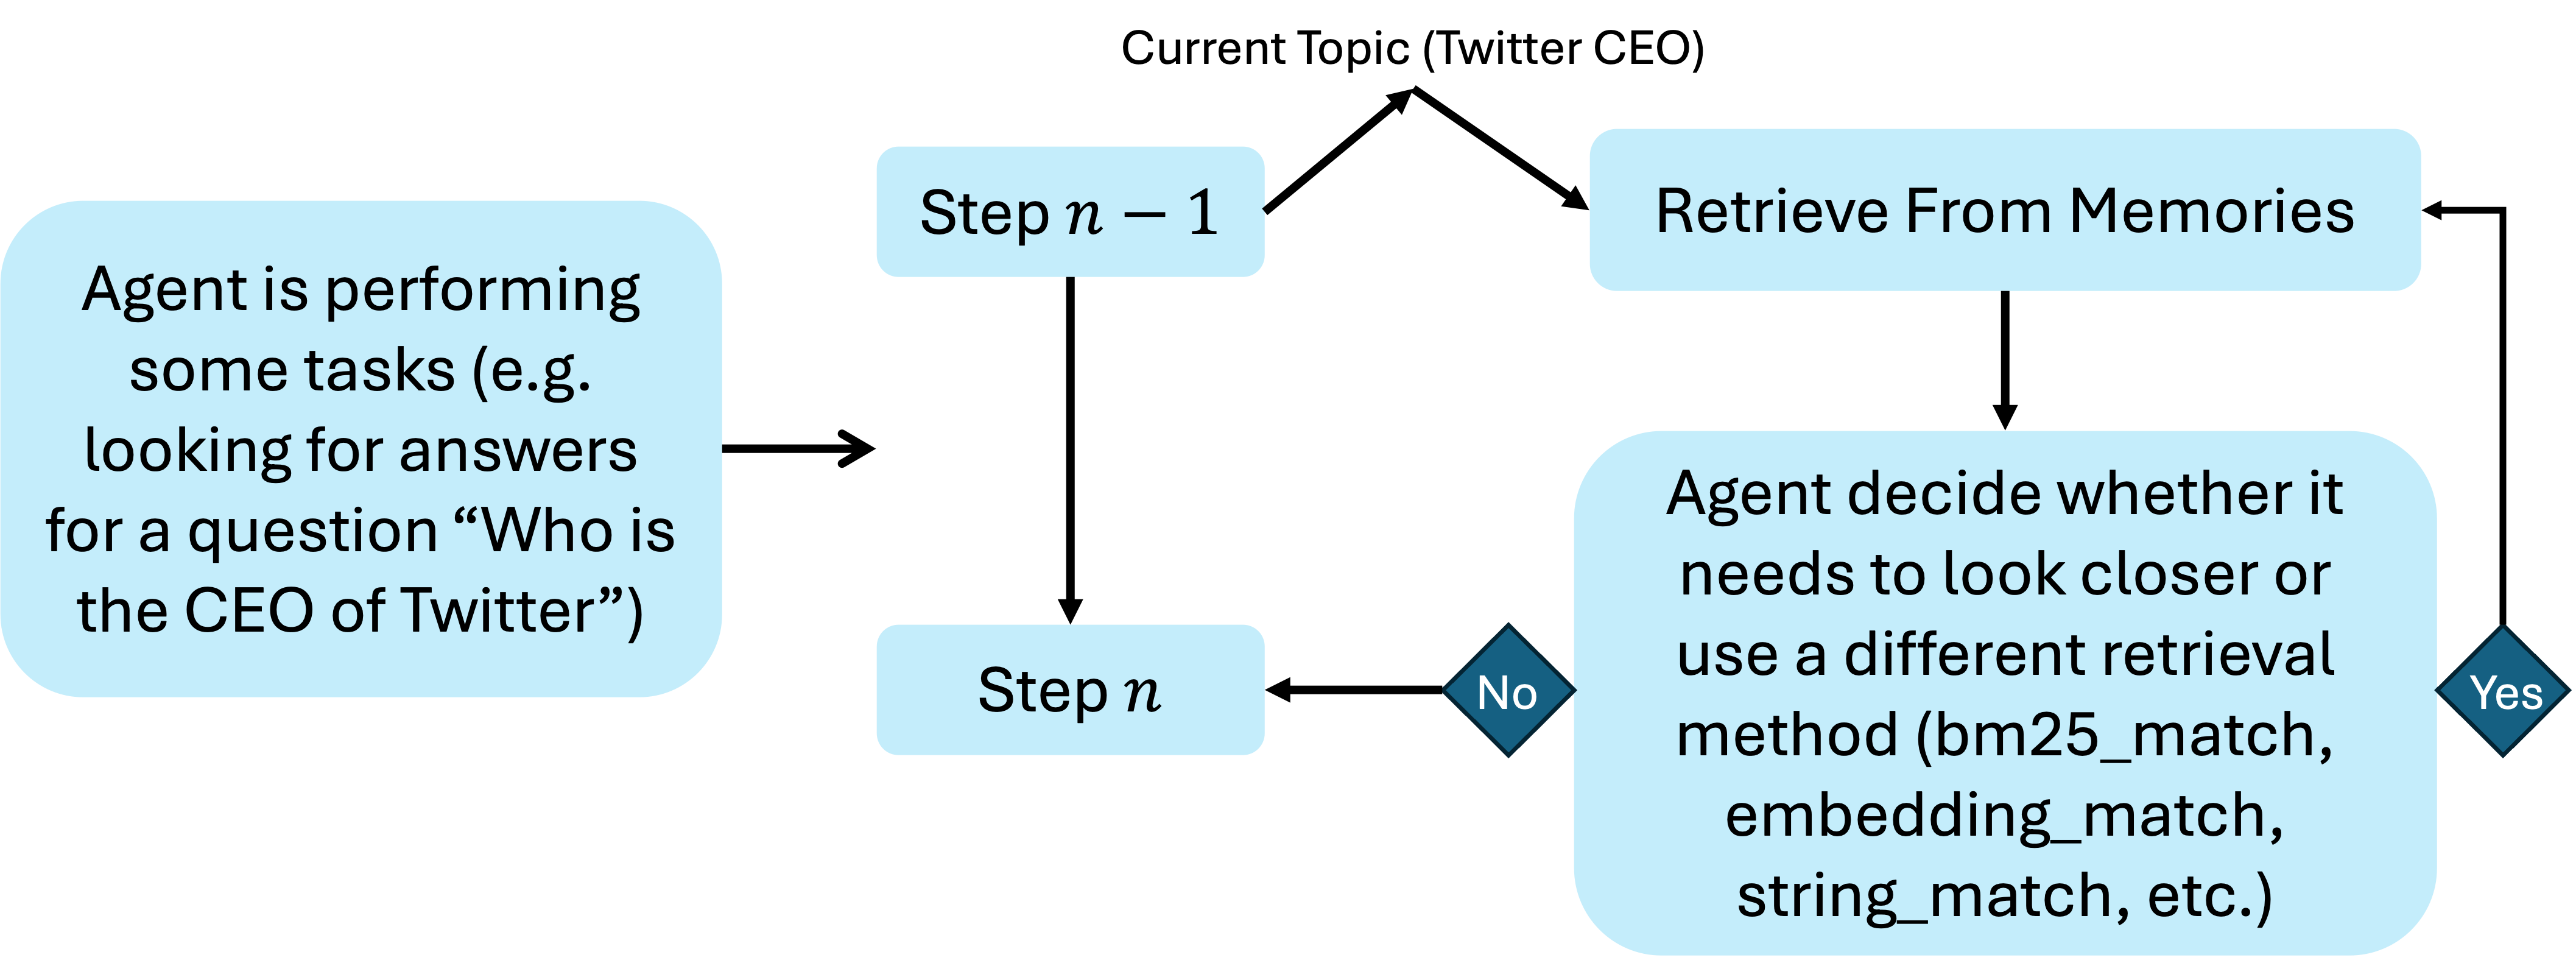
\includegraphics[width=0.8\linewidth]{figures/active_retrieval.png}
    \caption{Demonstration of Active Retrieval.}
    \label{fig:active_retrieval}
\end{figure}

\paragraph{Procedural Memory} 
Procedural Memory stores structured, goal-directed processes such as how-to guides, operational workflows, and interactive scripts. These are neither time-sensitive (episodic) nor abstract facts (semantic) but instead represent actionable knowledge that can be invoked to assist the user with complex tasks. Typical examples include ``how to file a travel reimbursement form,'' ``steps to set up a Zoom meeting,'' or ``how to book a restaurant via OpenTable.'' Each entry includes an \texttt{entry\_type} (\texttt{workflow}, \texttt{guide}, or \texttt{script}), a \texttt{description} of the goal or function, and \texttt{steps} expressed as a list of instructions (optionally in JSON or structured format). This memory component supports instructional planning, automation, and decomposition of user goals into sub-tasks.

\paragraph{Resource Memory} 
Resource Memory handles full or partial documents, transcripts, or multi-modal files that the user is actively engaged with but do not fit into other memory categories. For instance, if the user is reading a friend's detailed picnic plan or a project proposal document, the agent can store and retrieve that information from Resource Memory. This component enables context continuity in long-running tasks. Each entry includes a \texttt{title} (resource name), \texttt{summary} (brief overview and context), \texttt{resource\_type} (e.g., \texttt{doc}, \texttt{markdown}, \texttt{pdf\_text}, \texttt{image}, \texttt{voice\_transcript}), and the full or excerpted \texttt{content}. This design enables the agent to reference previously seen material, quote from documents, or search within them to aid the user’s workflow.

\paragraph{Knowledge Vault} 
The Knowledge Vault serves as a secure repository for verbatim and sensitive information such as credentials, addresses, contact information, and API keys. These entries are not typically relevant to conversation-level reasoning but are crucial for performing authenticated tasks or storing long-term identifiers. Each entry includes an \texttt{entry\_type} (e.g., \texttt{credential}, \texttt{bookmark}, \texttt{contact\_info}, \texttt{api\_key}), a \texttt{source} (e.g., \texttt{user\_provided}, \texttt{github}), a \texttt{sensitivity} level (\texttt{low}, \texttt{medium}, \texttt{high}), and the actual \texttt{secret\_value}. Entries with high sensitivity are protected via access control and excluded from casual retrieval to prevent misuse or leakage.

\subsection{Active Retrieval and Retrieval Design}
In many memory-augmented systems (e.g., Mem0~\citep{mem0}, MemGPT~\citep{memgpt}), memory retrieval must be explicitly triggered. Otherwise, the language model often defaults to its parametric knowledge, which may be outdated or incorrect. For example, suppose the user previously said, “The CEO of Twitter is Linda Yaccarino,” and this information was saved in memory. A few days later, when this message is no longer present in the conversation history, the user might ask, “Who is the CEO of Twitter?” In this case, the language model may rely on outdated knowledge and incorrectly respond with “Elon Musk.” While explicitly instructing the model to “search your memory” can mitigate such errors, doing so repeatedly is impractical in natural conversations.

\begin{figure}
    \centering
    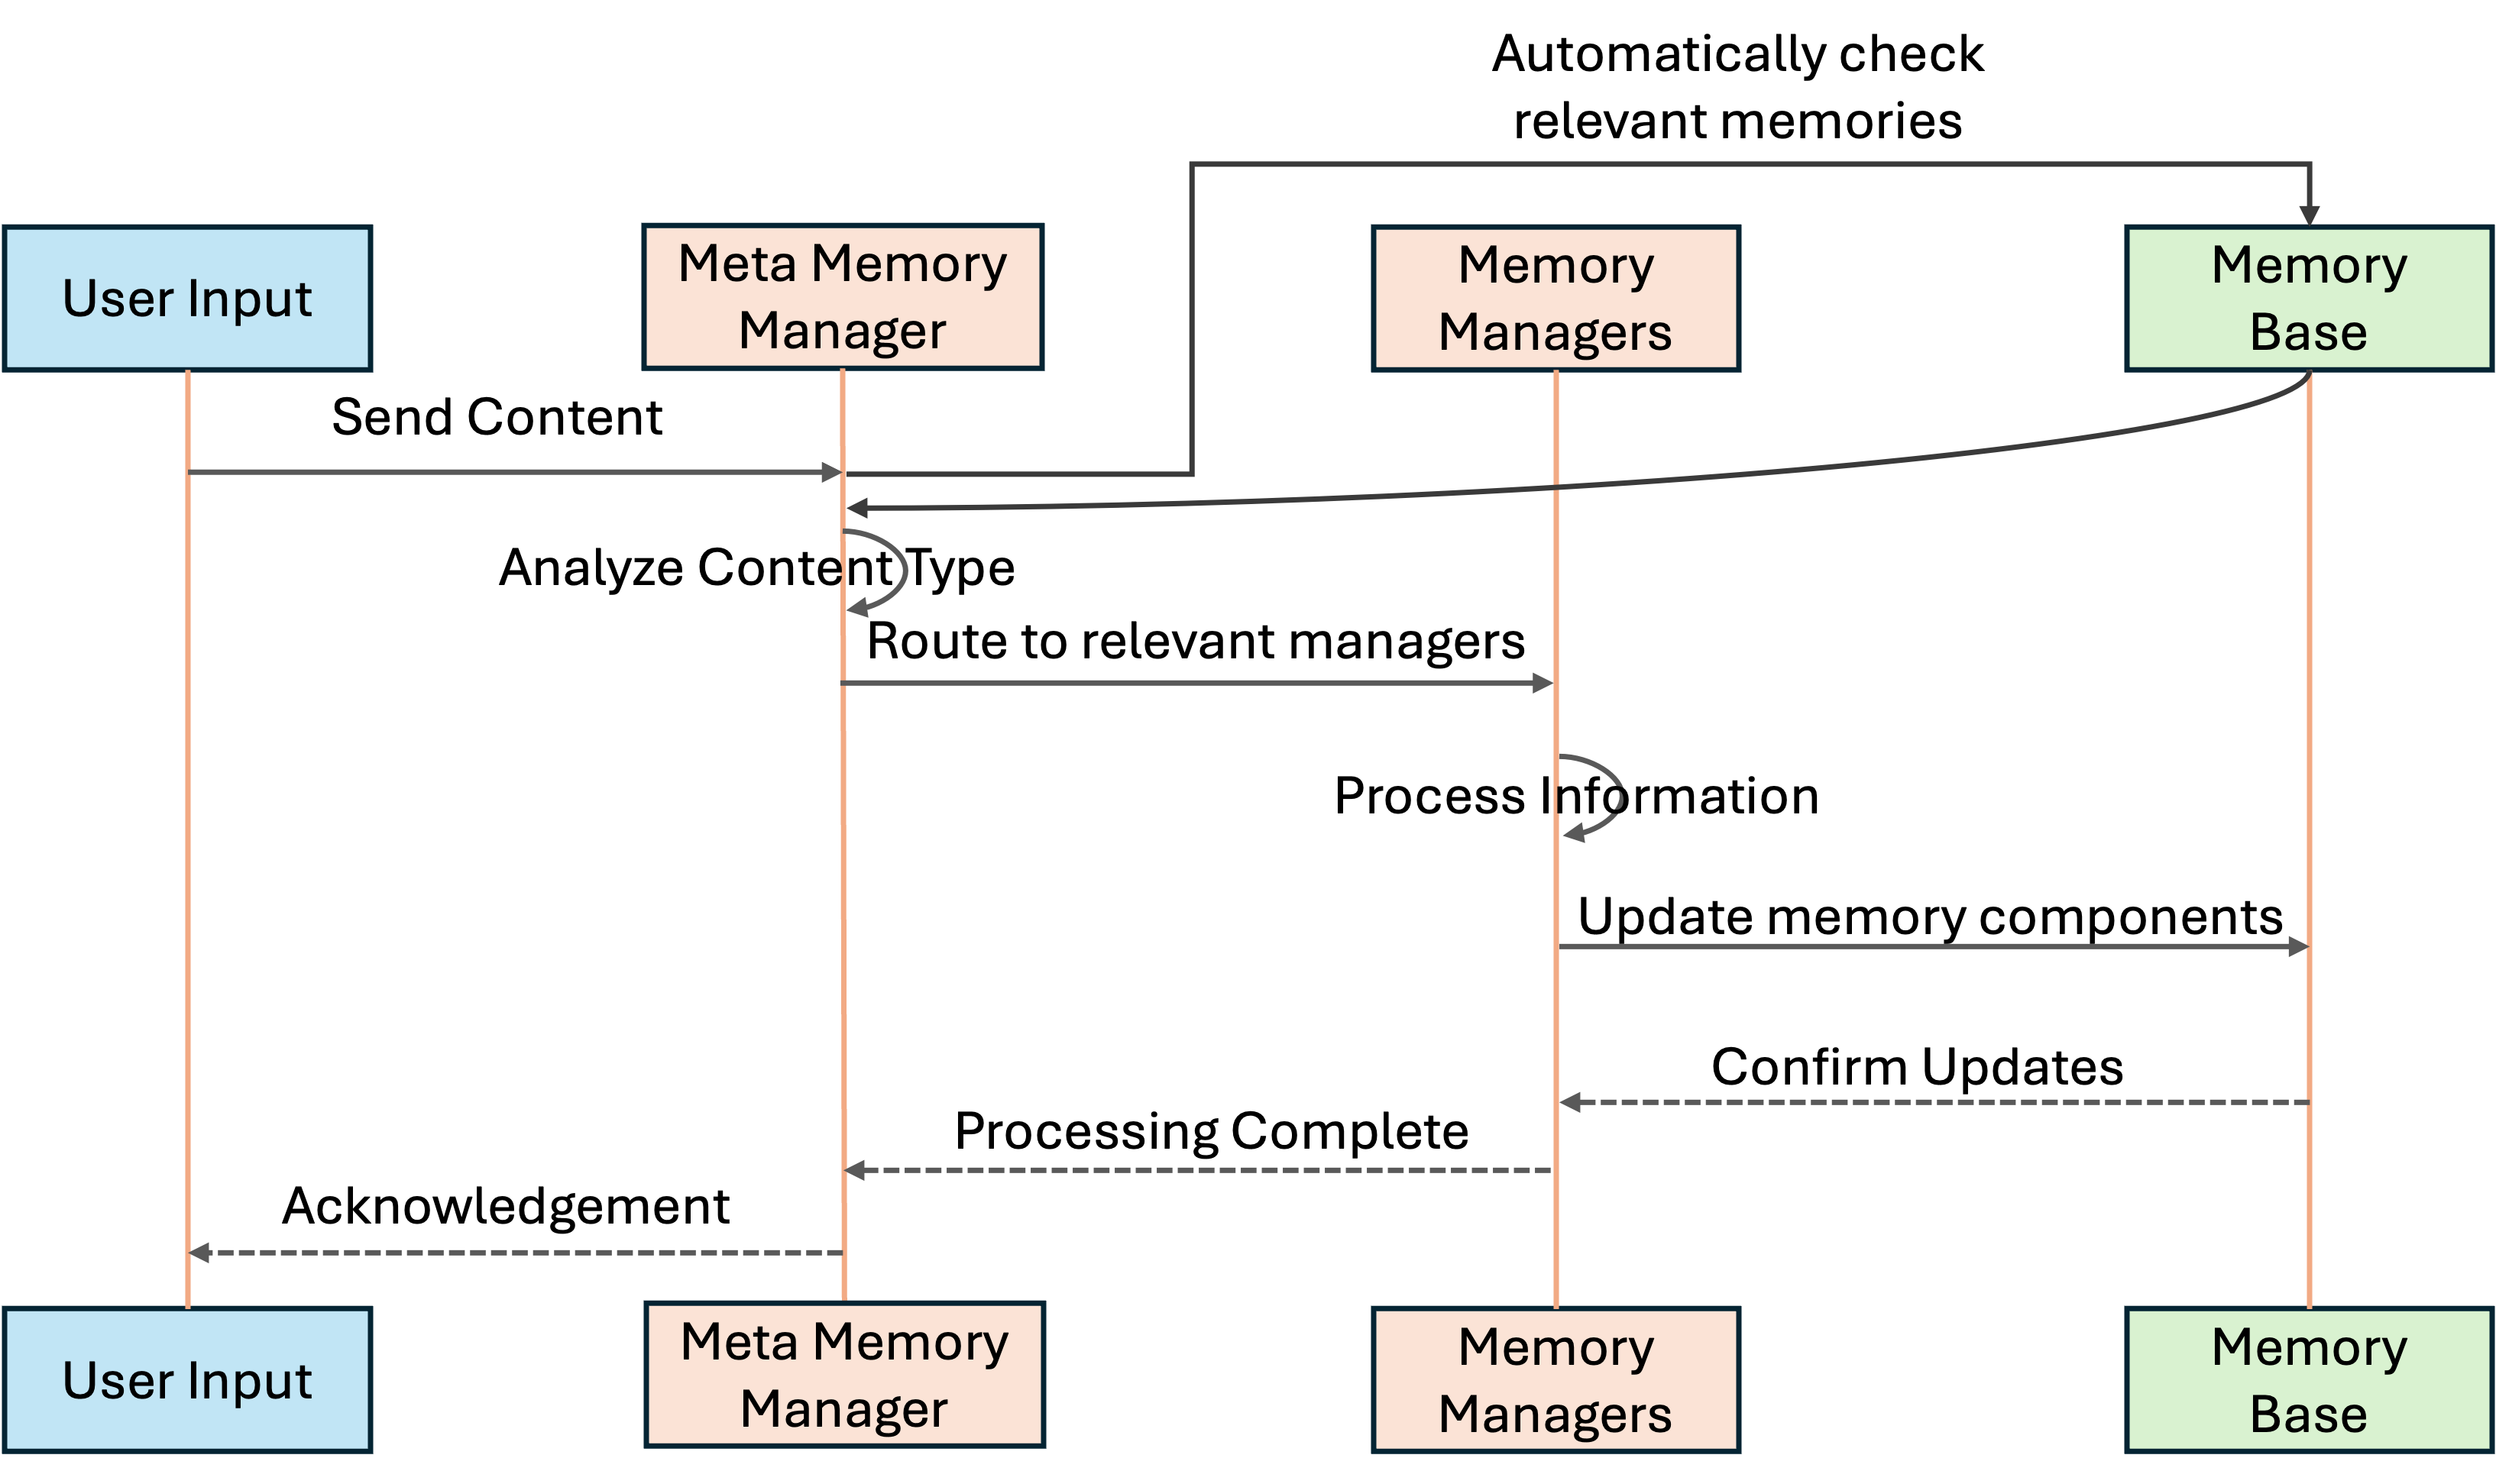
\includegraphics[width=\linewidth]{figures/update_workflow.png}
    \caption{The Workflow of Memory Update.}
    \label{fig:memory_update_workflow}
\end{figure}

To address this, we propose an \textbf{Active Retrieval} mechanism. As illustrated in Figure~\ref{fig:active_retrieval}, the system operates in two stages: first, the agent generates a \emph{current topic} based on the input context; second, this topic is used to retrieve relevant memories from each memory component. Retrieved results are then injected into the system prompt. For instance, given the query “Who is the CEO of Twitter?”, the agent may infer the topic “CEO of Twitter”, which is then used to retrieve the top-10 most relevant entries from each of the six memory components. Retrieved content is tagged according to its source, such as \texttt{<episodic\_memory>}... \texttt{</episodic\_memory>}, ensuring the model is aware of both the content and its origin. This automatic retrieval pipeline eliminates the need for explicit user prompts to trigger memory access and ensures the model can incorporate up-to-date, personalized, or contextual information during response generation.

In addition to Active Retrieval, we support multiple retrieval functions, including \texttt{embedding\_match}, \texttt{bm25\_match}, and \texttt{string\_match}. We are actively expanding this set with more diverse and specialized retrieval strategies, ensuring that each method is well-differentiated so the agent can choose the most appropriate one to invoke based on context.


\subsection{Multi-Agent Workflow}

To manage the dynamic and heterogeneous nature of user interactions, we adopt a modular multi-agent architecture. This system orchestrates input processing, memory updating, and information retrieval across six distinct memory components through a coordinated and efficient workflow. The overall system is governed by a central \textit{Meta Memory Manager} and a set of specialized \textit{Memory Managers}, each responsible for maintaining one memory type. 


\paragraph{Memory Update Workflow}
As illustrated in Figure~\ref{fig:memory_update_workflow}, when new input is received from the user, the system first automatically performs a search over the memory base. The retrieved information, together with the user input, is passed to the \emph{Meta Memory Manager}. The \emph{Meta Memory Manager} then analyzes the content and determines which memory components are relevant, routing the input to the corresponding \emph{Memory Managers}. These \emph{Memory Managers} update their respective memories in parallel while ensuring that redundant information is avoided within each memory type. After completing the updates, they report back to the \emph{Meta Memory Manager}, which finally sends an acknowledgment confirming that the memory update process is complete.

\paragraph{Conversational Retrieval Workflow}
For interactive dialogues, the \textit{Chat Agent} manages natural language communication with the user. To ground its responses in prior knowledge, it first performs an automatic search over the memory base upon receiving a user query. This initial search is a coarse retrieval spanning all six memory components and returns high-level summaries rather than detailed content. The Chat Agent then analyzes the query to determine which memory components warrant more targeted searches and selects appropriate retrieval methods accordingly. After obtaining the relevant results, it consolidates the information and synthesizes the final response. Moreover, if the user’s query involves updating memory—for example, providing new facts or corrections-the Chat Agent can interact directly with the corresponding Memory Managers to apply precise updates to specific memory components.
